\documentclass[tikz,border=10pt]{standalone}
\usepackage[T1]{fontenc}
\usepackage{lmodern}
\usepackage{amsmath}
\usetikzlibrary{arrows.meta,positioning,fit,backgrounds}

\definecolor{navy}{HTML}{17324D}
\definecolor{bluefill}{HTML}{EDF6FC}
\definecolor{purplefill}{HTML}{F1EDFC}
\definecolor{amberfill}{HTML}{FFF4DD}

\begin{document}
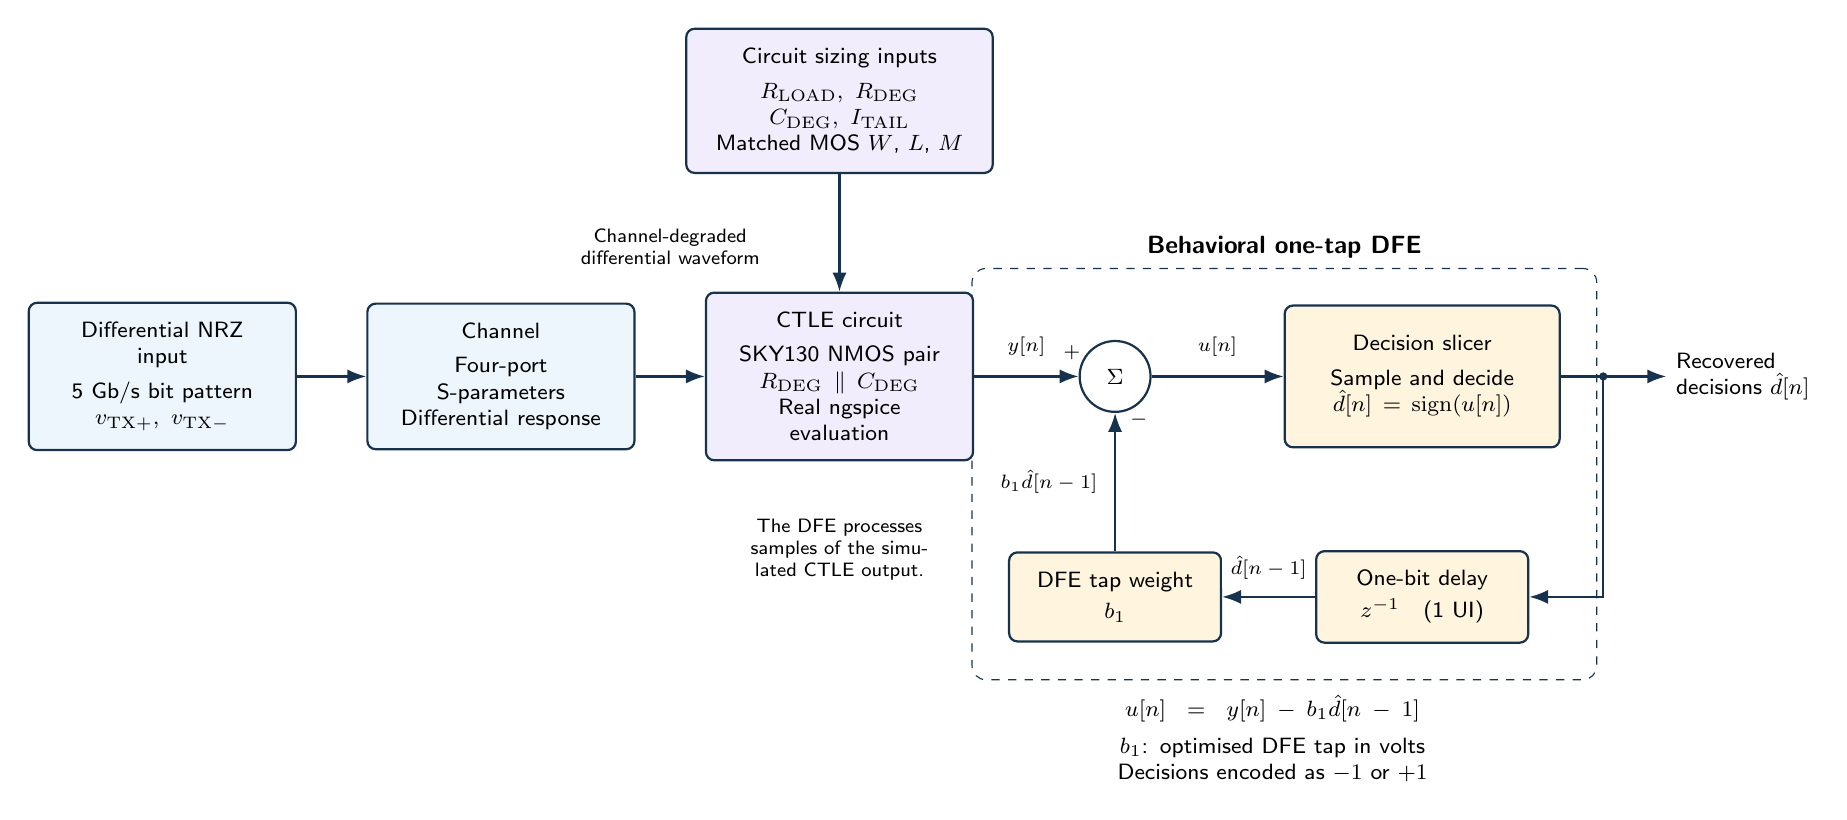
\begin{tikzpicture}[
  font=\sffamily\footnotesize,
  flow/.style={-{Latex[length=2.4mm]},thick,draw=navy},
  block/.style={draw=navy,thick,rounded corners=3pt,
    minimum height=1.8cm,text width=2.9cm,align=center,inner sep=7pt},
  tag/.style={font=\sffamily\scriptsize,align=center,fill=white,inner sep=3pt}
]

% Main signal path. Fixed coordinates leave space for labels and feedback.
\node[block,fill=bluefill] (input) at (0,0)
  {Differential NRZ\\input\\[3pt]5 Gb/s bit pattern\\$v_{\mathrm{TX}+},\ v_{\mathrm{TX}-}$};
\node[block,fill=bluefill] (channel) at (4.3,0)
  {Channel\\[3pt]Four-port\\S-parameters\\Differential response};
\node[block,fill=purplefill] (ctle) at (8.6,0)
  {CTLE circuit\\[3pt]SKY130 NMOS pair\\$R_{\mathrm{DEG}}\parallel C_{\mathrm{DEG}}$\\Real ngspice\\evaluation};
\node[circle,draw=navy,thick,minimum size=9mm,inner sep=0pt] (sum) at (12.1,0) {$\Sigma$};
\node[block,fill=amberfill,text width=3cm] (slicer) at (16,0)
  {Decision slicer\\[3pt]Sample and decide\\$\hat d[n]=\operatorname{sign}\!\left(u[n]\right)$};
\coordinate (branch) at (18.3,0);
\node[align=left,font=\sffamily\footnotesize,anchor=west] (output) at (19.1,0)
  {Recovered\\decisions $\hat d[n]$};

\draw[flow] (input) -- (channel);
\draw[flow] (channel) -- (ctle);
\node[tag,text width=2.5cm] at (6.45,1.65)
  {Channel-degraded\\differential waveform};
\draw[flow] (ctle) -- node[tag,above=4pt]{$y[n]$} (sum);
\draw[flow] (sum) -- node[tag,above=4pt]{$u[n]$} (slicer);
\draw[flow] (slicer) -- (output.west);
\node[font=\sffamily\scriptsize] at (11.55,0.3) {$+$};
\node[font=\sffamily\scriptsize] at (12.4,-0.55) {$-$};

% One previous decision is delayed and weighted before subtraction.
\node[block,fill=amberfill,text width=2.2cm,minimum height=1.1cm] (delay) at (16,-2.8)
  {One-bit delay\\[2pt]$z^{-1}$\quad (1 UI)};
\node[block,fill=amberfill,text width=2.2cm,minimum height=1.1cm] (tap) at (12.1,-2.8)
  {DFE tap weight\\[2pt]$b_1$};
\fill[navy] (branch) circle (1.5pt);
\draw[flow] (branch) |- (delay.east);
\draw[flow] (delay) -- node[tag,above=3pt]{$\hat d[n-1]$} (tap);
\draw[flow] (tap.north) -- node[tag,left=3pt]{$b_1\hat d[n-1]$} (sum.south);

% Parameter input to the physical circuit.
\node[block,fill=purplefill,text width=3.4cm,minimum height=1.2cm] (parameters) at (8.6,3.5)
  {Circuit sizing inputs\\[3pt]$R_{\mathrm{LOAD}},\ R_{\mathrm{DEG}}$\\$C_{\mathrm{DEG}},\ I_{\mathrm{TAIL}}$\\Matched MOS $W$, $L$, $M$};
\draw[flow] (parameters) -- (ctle);
\node[tag,text width=3.1cm] at (8.6,-2.2)
  {The DFE processes samples of the simulated CTLE output.};

\begin{scope}[on background layer]
  \node[draw=navy,dashed,rounded corners=5pt,
    fit=(sum)(slicer)(delay)(tap),inner sep=13pt] (dfebox) {};
\end{scope}
\node[anchor=south,font=\sffamily\bfseries\small] at (dfebox.north)
  {Behavioral one-tap DFE};
\node[align=center,text width=6.4cm,font=\sffamily\footnotesize] at (14.1,-4.6)
  {$u[n]=y[n]-b_1\hat d[n-1]$\\[4pt]
   $b_1$: optimised DFE tap in volts\\Decisions encoded as $-1$ or $+1$};

\end{tikzpicture}
\end{document}
